We now consider an elastic solid with square section of dimension $l=3m$ in the ($\vect{e}_1,\vect{e}_2$) plane, and infinite in the direction $\vect{e}_3$ so that the plane strain assumption (\textit{i.e. $\eps_{33}=\eps_{13}=\eps_{23}=0$}) holds. The values of elastic parameters considered are still those of table \ref{tab:material}. The solid suddenly undergoes a tensile stress on a part of its left boundary (see figure \ref{fig:2D_planeStrain}\subref{subfig:2D_problem}) so that shear and pressure waves travel in the mediumtoward the horizontally fixed right end, reflect and then propagate leftward.
\begin{figure}[h!]
  \centering
  \subcaptionbox{Geometry and boundary conditions\label{subfig:2D_problem}}{\begin{tikzpicture}[scale=0.9]
  \draw[thick] (0,0) --(3,0)--(3,3)--(0,3)--(0,0);
  \foreach \x in {0.5,1.,...,2.5} 
  \draw(\x,-0.2)circle(0.2);
  \foreach \x in {0.25,0.75,...,2.75} 
  \draw(3.2,\x)circle(0.2);
  \draw(0,-0.4)--(3.,-0.4);
  \draw(3.4,0)--(3.4,3);
  \fill [pattern=north east lines](0.0,-0.8)rectangle+(3,0.4);
  \fill [pattern=north east lines](3.4,0.)rectangle+(0.4,3);
  \draw[>=stealth,<->](0,3.1)--node[above=1pt]{\footnotesize $l=3 \: m$}(3,3.1);
  \draw[>=stealth,<->](0.1,0)--node[right=1pt]{\footnotesize $a=1 \: m$}(0.1,1);
  \foreach \x in {0.,0.25,...,1} 
  \draw[>=stealth,<-] (-0.5,\x)--(0.,\x);
  \node(a)at(-1.75,0.5){\footnotesize $\tens{\sigma}\cdot\vect{e}_1=\matrice{\sigma^d\\0 \\0}$}; 
  \draw[>=stealth,->](-1.5,2)--(-0.5,2)node(a)[anchor=north]{\footnotesize $\vect{e}_1$};
  \draw[>=stealth,->](-1.5,2)--(-1.5,3)node(a)[anchor=south]{\footnotesize $\vect{e}_2$};
\end{tikzpicture}


%%% Local Variables:
%%% mode: latex
%%% TeX-master: "../../mainManuscript"
%%% End:
} \qquad
  \subcaptionbox{Material points set and grids \label{subfig:2d_meshes}}{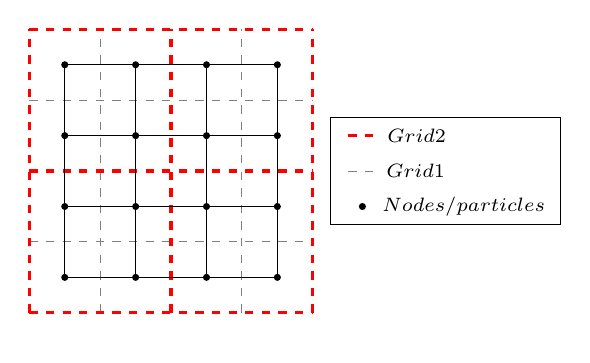
\begin{tikzpicture}[scale=0.9]
  \draw (0,0) --(3,0)--(3,3)--(0,3)--(0,0);
  \draw[white] (0.,0) -- (0,-0.8);
  %%% Grid 1
  \foreach \y in {-0.5,0.5,...,3.5} 
  \draw[dashed,gray] (-0.5,\y) -- (3.5,\y);
  \foreach \x in {-0.5,0.5,...,3.5} 
  \draw[dashed,gray] (\x,-0.5) -- (\x,3.5);
  %%% Grid 2
  \foreach \y in {-0.5,1.5,...,3.5} 
  \draw[dashed,Red,very thick] (-0.5,\y) -- (3.5,\y);
  \foreach \x in {-0.5,1.5,...,3.5} 
  \draw[dashed,Red,very thick] (\x,-0.5) -- (\x,3.5);
  \foreach \y in {0.,1.,...,3.} 
  \foreach \x in {0.,1.,...,3.} 
  \fill (\x,\y) circle(0.05);
  \foreach \y in {0.,1.,...,3.} 
  \draw (0,\y) -- (3.,\y);
  \foreach \x in {0.,1.,...,3.} 
  \draw (\x,0) -- (\x,3);
  \draw (3.75,0.75) rectangle (7.,2.25);
  \fill (4.2,1.) circle (0.05) node [right] {\scriptsize$ \: \: \text{Nodes / particles}$};
  \draw[dashed,gray] (4.,1.5) -- (4.4,1.5) node [right] {\scriptsize$\color{black} \text{Grid 1}$};
  \draw[dashed,very thick,Red] (4.,2.) -- (4.4,2.) node [right] {\scriptsize$\color{black} \text{Grid 2}$};
\end{tikzpicture}


%%% Local Variables:
%%% mode: latex
%%% TeX-master: "../manuscript"
%%% End:
}
  \caption{Geometry, loading and boundary conditions for the tensile impact problem on a two-dimensional elastic medium.}
  \label{fig:2D_planeStrain}
\end{figure}
The exact solution of this problem being unknown, DGMPM solutions using the CTU method are compared to the MPM solution and to $Q1$ finite element (bilinear approximation) solutions obtained with the code Cast3M Drexus \cite{Castem}.

The solid is discretized such that material points are equivalent to finite element nodes, that is: $l\times l \equiv 28 \times 28$ particles and nodes. Moreover, two arbitrary grids are used for the DGMPM so that either one of four material points lie in every cells as depicted in figure \ref{fig:2D_planeStrain}\subref{subfig:2d_meshes} for a coarse example.
Figure \ref{fig:2delast_comparison} shows the isovalues of longitudinal stress $\sigma_{11}$ in the two-dimensional medium resulting from every numerical methods stated above at two different times with the traction force set to $\sigma^d=200\: Mpa$. The first and second lines of plots respectively corresponds to the stress profile before and after reflection of the pressure wave on the right boundary of the domain.
Unlike FEM and MPM, the DGMPM does not exhibit oscillations regardless of the number of particles in grid cells. Nevertheless, the decrease in the CFL number involved by the 4ppc discretization yield a less accurate resolution of the jump discontinuity carried by the longitudinal pressure wave than for 1ppc.
\begin{figure}[h!]
  \centering
  \begin{tikzpicture}
  \begin{groupplot}[group style={group size=4 by 2,
      ylabels at=edge left, yticklabels at=edge left,
      horizontal sep=1.ex,
      vertical sep=2ex,},
    enlargelimits=0,
    xmin=0.,xmax=1., ymin=-0.,ymax=1.
    ,axis on top,scale only axis,xtick=\empty,ytick=\empty,width=0.2\linewidth,
    colorbar style={
      title style={
        font=\scriptsize,
        at={(1,.25)},
        anchor=north west
      },yticklabel style={font=\scriptsize}
      ,at={(current axis.south east)},anchor=south west
    }]
    %% FIRST ROW (time 1 = 3.5e-4s)
    %%% RANGE -2.0e7 -- 2.9e8
    \nextgroupplot[ylabel={$t=3.5\times 10^{-4} \:s$},title={(a) FEM}]\addplot graphics[xmin=0.,xmax=1., ymin=-0.,ymax=1.] {chapter4/pngFigures/fem_stress_115.png};
    \nextgroupplot[title={(b) DGMPM 1ppc}]\addplot graphics[xmin=-0.,xmax=1., ymin=-0.,ymax=1.] {chapter4/pngFigures/dgmpm1ppc_stress_115.png};
    \nextgroupplot[title={(c) DGMPM 4ppc}]\addplot graphics[xmin=-0.,xmax=1., ymin=-0.,ymax=1.] {chapter4/pngFigures/dgmpm4ppc_stress_115.png};
    \nextgroupplot[title={(d) MPM 1ppc},
    colorbar,colorbar style={
      title= {$\sigma_{11}\: (MPa)$},
      ytick={-5.7e-2,2.e-1,2.9e-1},
      yticklabels={-57,200,290},
    }]
    \addplot[scatter,scatter src=y,mark size=0.pt] coordinates {(0.,-5.7e-2) (0.,2.9e-1)};% Fake extreme values to fix scale
    \addplot graphics[xmin=-0.,xmax=1., ymin=-0.,ymax=1.] {chapter4/pngFigures/mpm_stress_115.png};

    %% SECOND ROW (time 2 =1.e-3s)
    %%% RANGE -4.4e7 -- 4.2e8
    \nextgroupplot[ylabel={$t=1.0\times 10^{-3} \:s$}]\addplot graphics[xmin=0.,xmax=1., ymin=-0.,ymax=1.] {chapter4/pngFigures/fem_stress_338.png};
    \nextgroupplot[]\addplot graphics[xmin=-0.,xmax=1., ymin=-0.,ymax=1.] {chapter4/pngFigures/dgmpm1ppc_stress_338.png};
    \nextgroupplot[]\addplot graphics[xmin=-0.,xmax=1., ymin=-0.,ymax=1.] {chapter4/pngFigures/dgmpm4ppc_stress_338.png};
    \nextgroupplot[colorbar,colorbar style={
      title= {$\sigma_{11}\: (MPa)$},
      ytick={-4.3e-2,2.e-1,4.8e-1},
      yticklabels={-43,200,480},
    }]
    \addplot[scatter,scatter src=y,mark size=0.pt] coordinates {(0.,-4.3e-2) (0.,4.8e-1)};% Fake extreme values to fix scale
    \addplot graphics[xmin=-0.,xmax=1., ymin=-0.,ymax=1.] {chapter4/pngFigures/mpm_stress_338.png};
    
  \end{groupplot}
\end{tikzpicture}



%%% Local Variables:
%%% mode: latex
%%% TeX-master: "../mainManuscript"
%%% End:

  \caption{Isovalues of longitudinal stress $\sigma_{11}$ solution of the tensile impact problem in a two-dimensional elastic medium. Comparison between FEM (CFL=0.9), DGMPM-CTU using 1ppc (CFL=1) or 4ppc (CFL=0.23), and MPM using 1ppc (CFL=0.7).}
  \label{fig:2delast_comparison}
\end{figure}
On the other hand, the propagation of waves in both directions $\vect{e}_1$ and $\vect{e}_2$ provides a cylindrical profile to the longitudinal stress that is almost indentically described by FEM and DGMPM using 1ppc, even after reflection of the fixed boundary (second row in figure \ref{fig:2delast_comparison}). The smoothness of the DGMPM solutions using 4ppc and the oscillations in MPM results prevent distinguishing this structure.

Note that this problem is solved in a two-dimensional setting in \cite{DGMPM} by considering an infinite medium in direction $\vect{e}_3$, of dimension $l\times h$ in directions $\vect{e}_1$ and $\vect{e}_2$, which bottom and top boundaries are assumed vertically fixed.
The results coming from the two-dimensional simulation using the CTU approach show a good agreement with the exact solution of the problem that is still valid. Hence, in what follows, a more general problem that that of a plane wave in considered.



%%% Local Variables:
%%% mode: latex
%%% TeX-master: "../mainManuscript"
%%% End:
